% !TeX spellcheck = cs_CZ
\begin{mathexam}{Z břevna kruhového průřezu s poloměrem \(r = \protect\SI{20}{\protect\cm}\) máme
  vytesat trám, který bude mít průřez ve tvaru obdélníka se stranami \(z\) a \(v\) („základnou“ a
  „výškou“). Jak máme volit \(z\) a \(v\), aby trám měl maximální nosnost, víme-li, že jeho nosnost
  je úměrná první mocnině \(z\) a druhé mocnině \(v\)?}{exam091}
   
  {\centering
    \captionsetup{type=figure}
    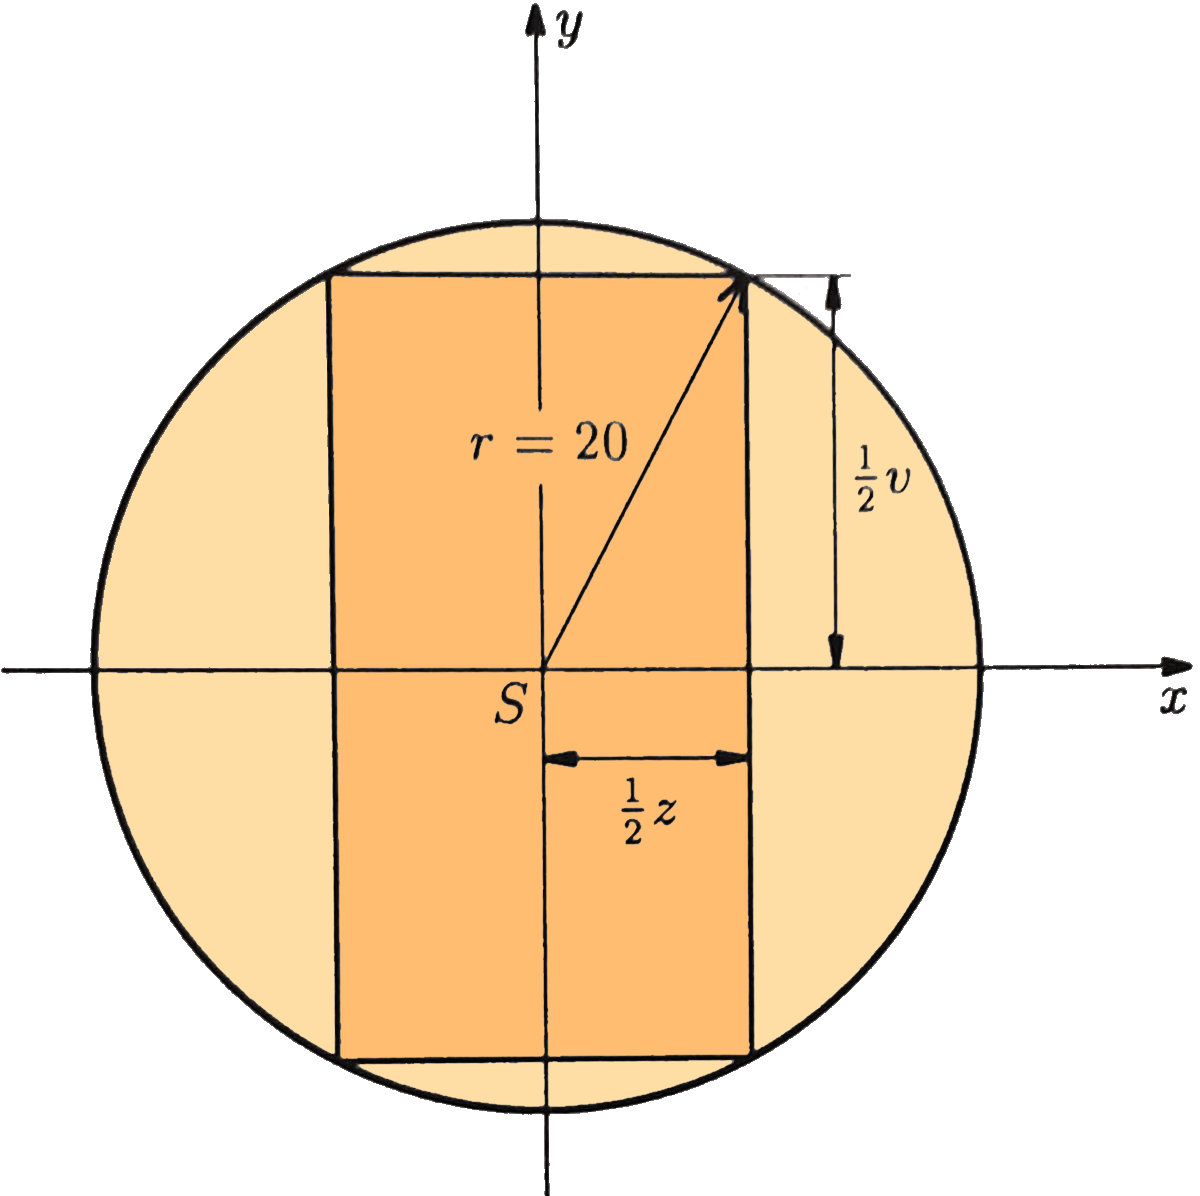
\includegraphics[width=1\linewidth]{mai_fig061.png} 
    \captionof{figure}{K příkladu \ref{mai:exam091}. Kredit: \cite[s.~47]{rektorys2011}}
    \label{mai:fig061}
  \par}
  
  Matematická formulace: Jaké rozměry má mít obdélník vepsaný do kružnice s poIoměrem \SI{20}{\cm},
  má-li být součin základny \(z\) a druhé mocniny výšky v maximální,
  \begin{equation*}
    y = z\cdot v^2 = ?
  \end{equation*}
  Zvolme za proměnnou z. Podle Pythagorovy věty platí (viz \ref{mai:fig061})
  \begin{equation*}
      r^2 = \left(\dfrac{z}{2}\right)^2 + \left(\dfrac{v}{2}\right)^2,
  \end{equation*}
  odkud 
  \begin{equation*}
      v^2 = 4r^2 - z^2.
  \end{equation*}
  Máme tedy najít maximum funkce
  \begin{equation}\label{mai:eq086}
      y = zv^2 = z(4r^2 - z^2) = 4r^2z - z^3,
  \end{equation}
  a to na intervalu \((0,40)\), neboť \(z\) nemůže být větší než \(2r = 40\). Ale funkce
  (\ref{mai:eq086}) je na tomto intervalu nezáporná a pro \(z = 0\) a \(z = 40\) je rovna nule
  (neboť pak \(4r^2 - z^2 = 0\). Hledáme tedy lokální maximum funkce (\ref{mai:eq086}) v otevřeném
  intervalu \(0,40)\). 

  Funkce (\ref{mai:eq086}) má všude první a druhou derivaci,
  \begin{equation*}
      y' = 4r^2 - 3z^2, \qquad\qquad y'' = -6z.
  \end{equation*}
  Může tedy předně nabývat v intervalu \((0, 40)\) lokálního extrému jen tam, kde je \(y'=0\), tj.
  kde
  \begin{equation*}
      4r^2 - 3z^2 = 0.
  \end{equation*}
  Odtud plyne, neboť má být \(z > 0\), že
  \begin{equation*}
      z = \sqrt{\dfrac{4r^2}{3}} = \dfrac{2}{\sqrt{3}}r = \dfrac{2\sqrt{3}}{3}r = 
          \dfrac{2\sqrt{3}}{3}20 \simeq \num{23.1}.
  \end{equation*}
  Pro \(v\) pak \(z\) dostaneme
  \begin{equation*}
      v = \sqrt{4r^2 - \dfrac{4}{3}r^2} = \sqrt{\frac{8}{3}\cdot20^2}\simeq\num{32.6}
  \end{equation*}
  V bodě \(z = \num{23.1}\) bude mít funkce (\ref{mai:eq086}) skutečně lokální maximum, a to ostré,
  neboť druhá derivace je v tomto bodě záporná.
\end{mathexam}